\section{Konzept} % Daniel
\begin{frame}
    \frametitle{Konzept}
    \begin{columns}
        \begin{column}{0.4\textwidth}
            \begin{block}{Teilkonzepte}
                \begin{itemize}
                    \item<2-> Korberkennung
                    \item<3-> Ausrichtung
                    \item<4-> Ballbeschleunigung
                    \item<5-> Ballnachführung
                    \item<6-> Kommunikation
                    \item<7-> Energieversorgung
                \end{itemize}
            \end{block}
        \end{column}
        \begin{column}{0.6\textwidth}
            \centering
            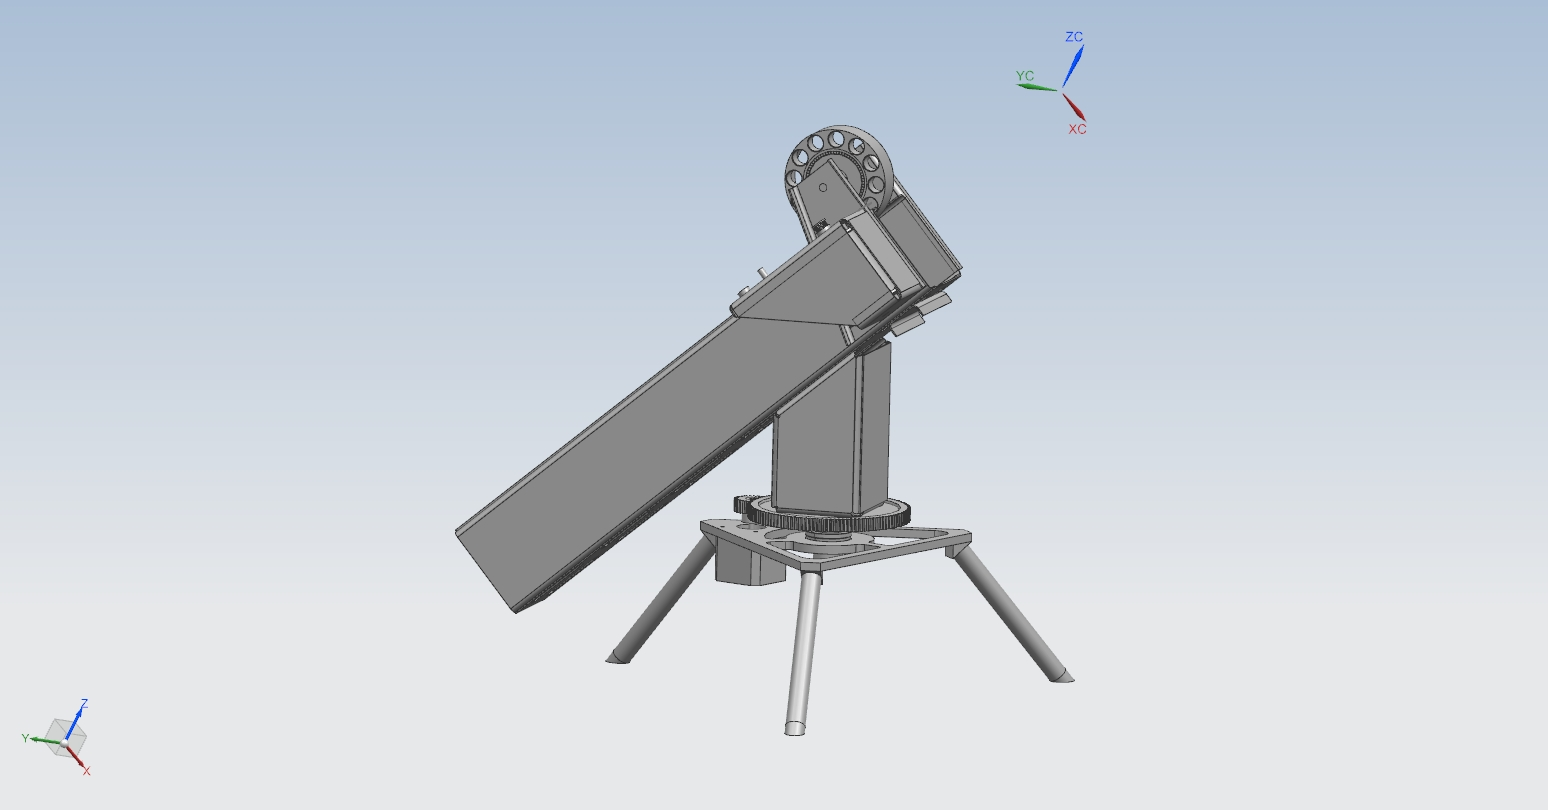
\includegraphics[width=0.8\textwidth, trim = 150mm 50 150mm 10, clip]{../doc/fig/Gesamt_bg1.jpg}
        \end{column}
    \end{columns}
\end{frame}

\begin{frame}
    \frametitle{Konzept}
    \framesubtitle{Korberkennung}
    \begin{columns}
        \begin{column}{0.4\textwidth}
            \begin{block}{Korberkennung}
                \begin{itemize}
                    \item Kamera
                    \item OpenCV
                \end{itemize}
            \end{block}
        \end{column}
        \begin{column}{0.6\textwidth}
        \end{column}
    \end{columns}
\end{frame}

\begin{frame}
    \frametitle{Konzept}
    \framesubtitle{Ausrichtung}
    \begin{columns}
        \begin{column}{0.4\textwidth}
            \begin{block}{Ausrichtung}
                \begin{itemize}
                    \item Drehung
                    \item Schrittmotor
                    \item Getriebe
                \end{itemize}
            \end{block}
        \end{column}
        \begin{column}{0.6\textwidth}
            \centering
            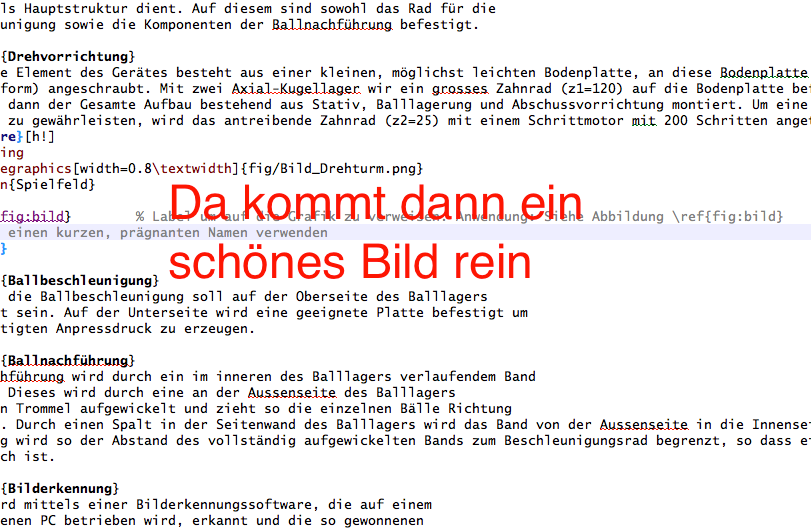
\includegraphics[width=1.0\textwidth, trim = 20mm 23mm 5mm 15mm, clip]{../doc/fig/Bild_Drehturm.png}
        \end{column}
    \end{columns}
\end{frame}

\begin{frame}
    \frametitle{Konzept}
    \framesubtitle{Ballbeschleunigung}
    \begin{columns}
        \begin{column}{0.4\textwidth}
            \begin{block}{Ballbeschleunigung}
                \begin{itemize}
                    \item Ein Rad oberhalb
                    \item<2-> BLDC Motor
                \end{itemize}
            \end{block}
            \centering
            \pause
            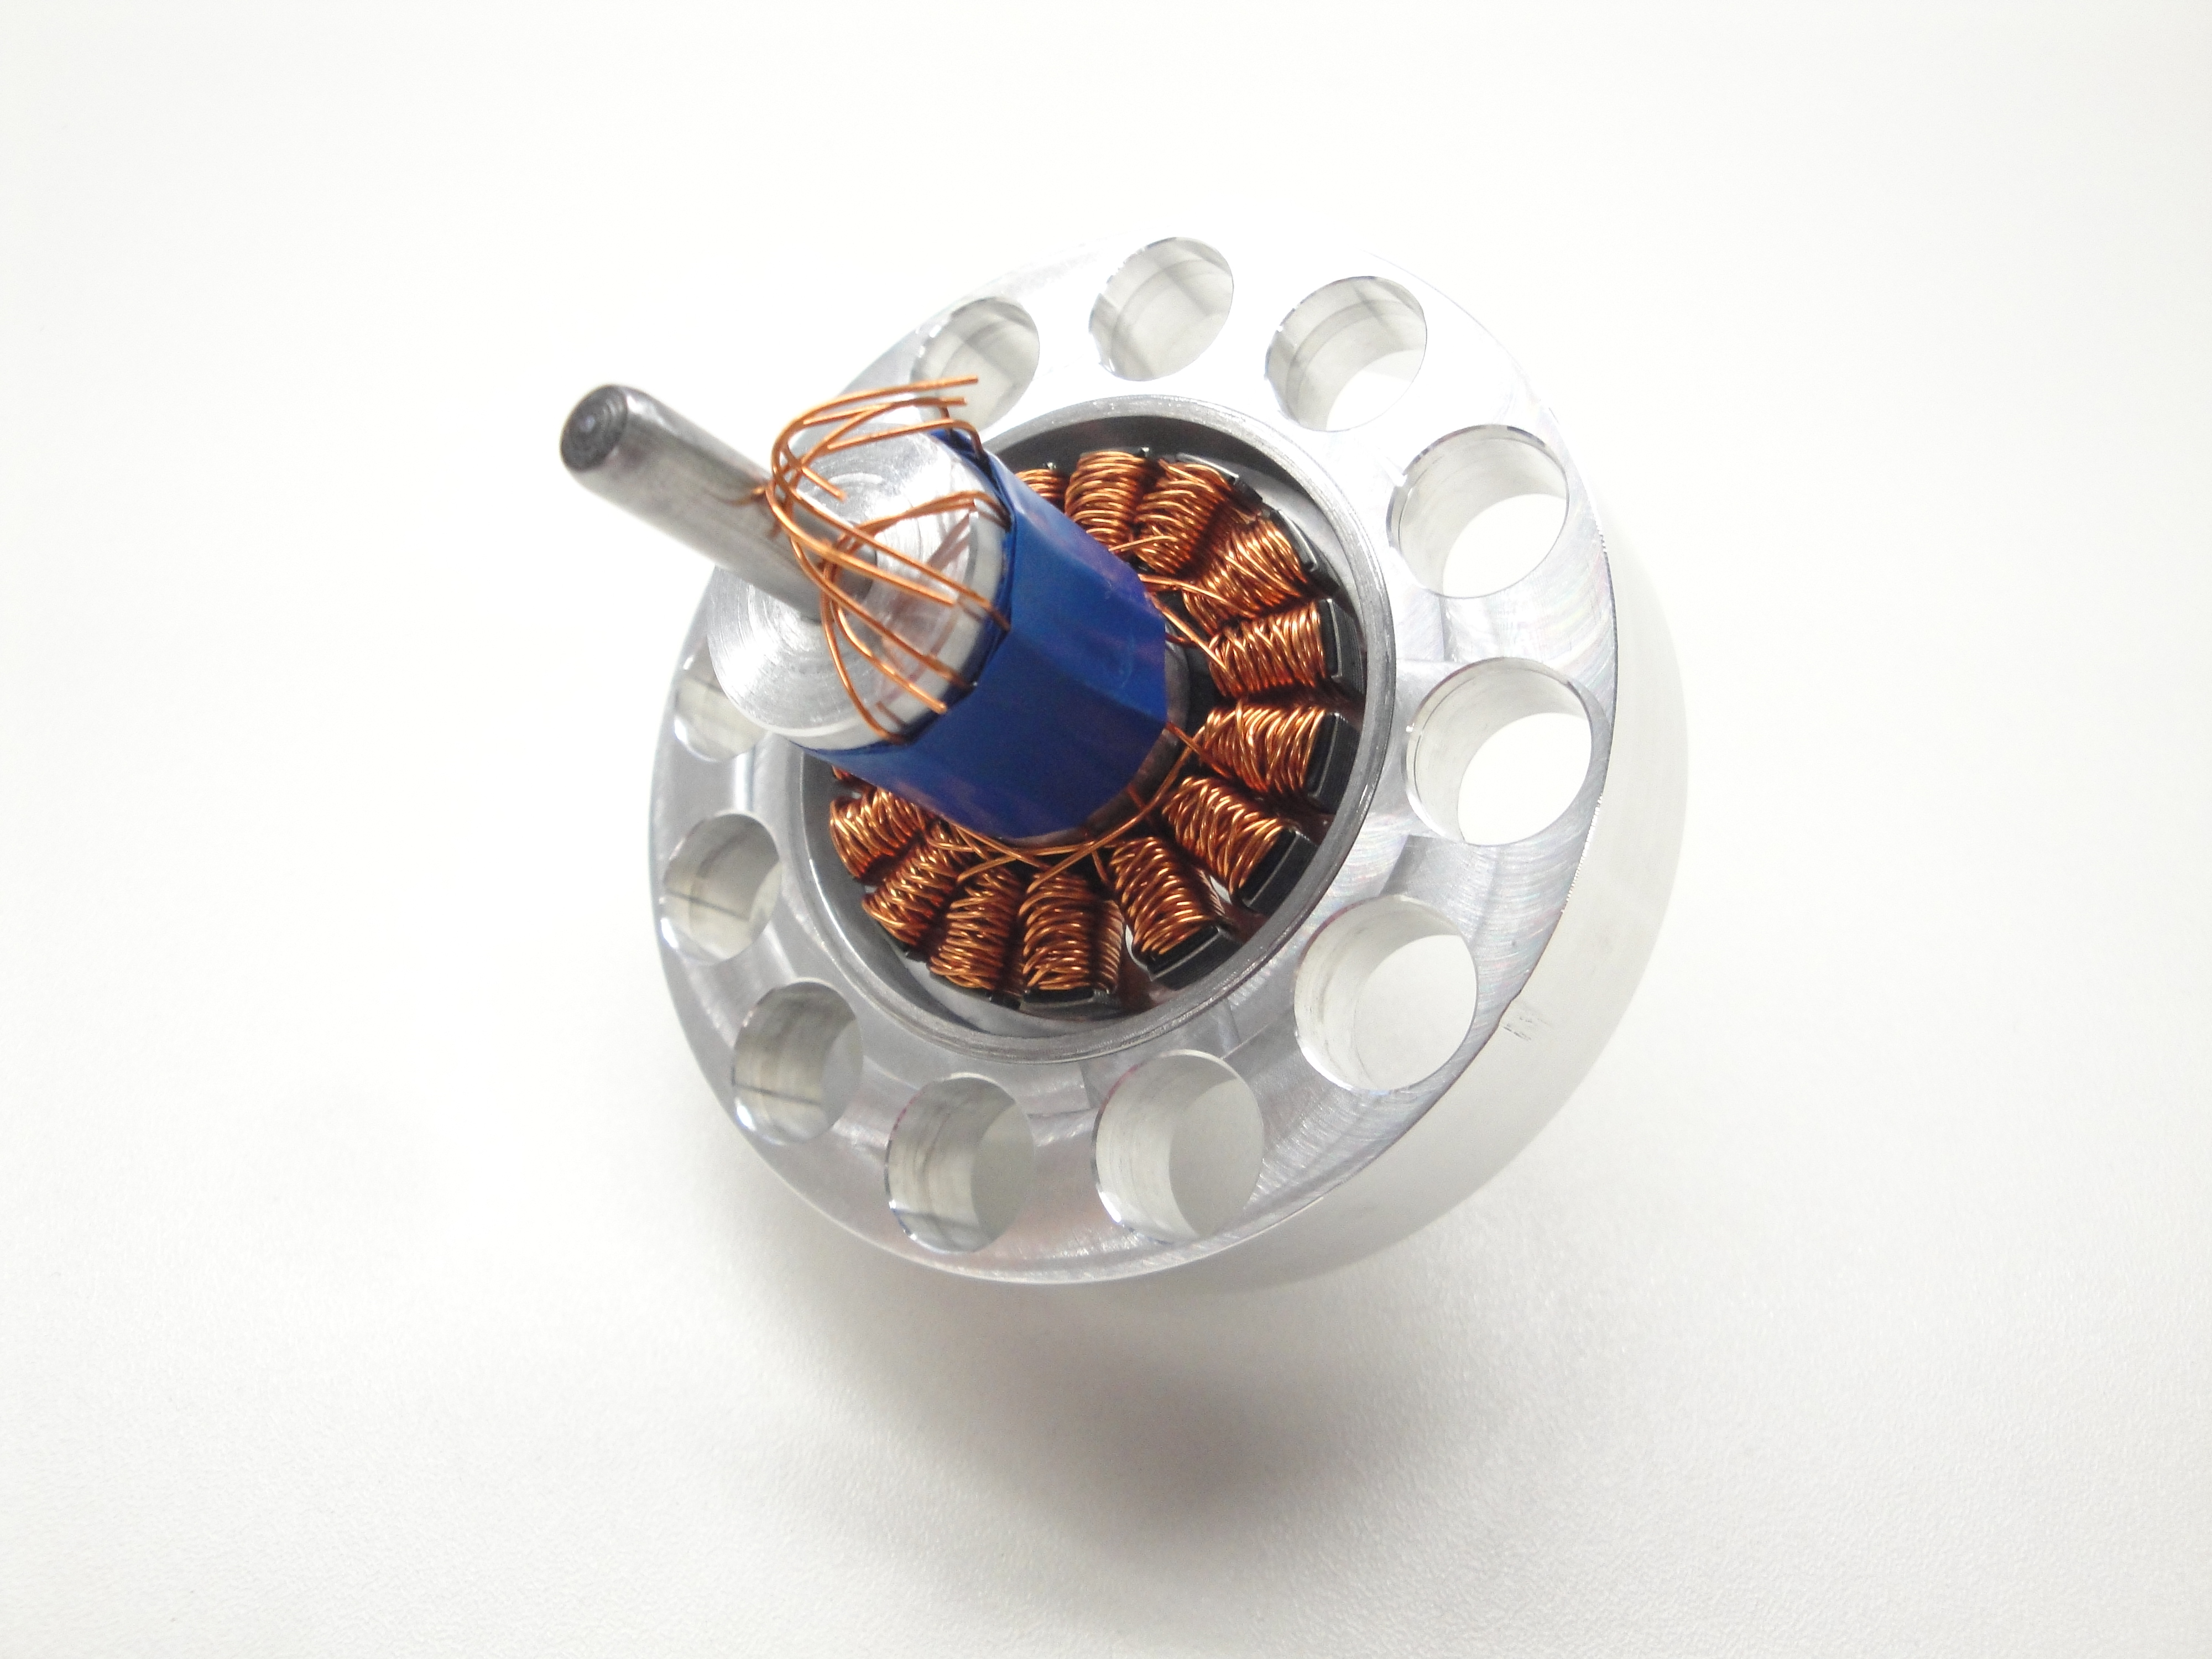
\includegraphics[width=0.8\textwidth, trim = 330mm 200mm 300mm 100mm, clip]{../fig/bldc/DSC02754.JPG}
        \end{column}
        \begin{column}{0.6\textwidth}
            \centering
            \onslide
            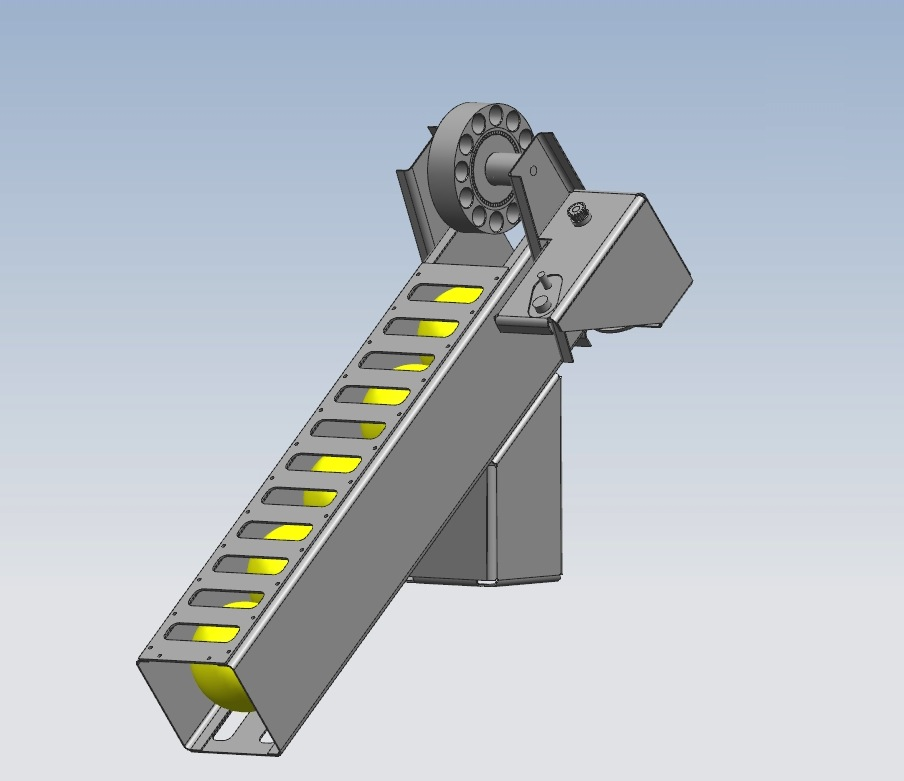
\includegraphics[width=0.8\textwidth, trim = 40mm 0mm 60mm 30mm, clip]{../doc/fig/Balllager.jpg}
        \end{column}
    \end{columns}
\end{frame}

\begin{frame}
    \frametitle{Konzept}
    \framesubtitle{Ballnachführung}
    \begin{block}{Ballnachführung}
        \begin{itemize}
            \item Stahlband
            \item DC Motor
        \end{itemize}
    \end{block}
\end{frame}

\begin{frame}
    \frametitle{Konzept}
    \framesubtitle{Kommunikation}
    \begin{block}{Kommunikation}
        \begin{itemize}
            \item Bluetooth für Steuerung
            \item WLAN für Kamerabild
        \end{itemize}
    \end{block}
\end{frame}

\begin{frame}
    \frametitle{Konzept}
    \framesubtitle{Energieversorgung}
    \begin{block}{Energieversorgung}
        \begin{itemize}
            \item Netzteil
            \item 24 \ldots 36 V
        \end{itemize}
    \end{block}
\end{frame}

